\documentclass{article}
\usepackage{graphicx} % Required for inserting images
\usepackage[a4paper, total={6in, 8in}]{geometry}
\usepackage{float} % Required for positioning figures and tables at the specified location

\title{CE4046 Intelligent Agent Assignment 1}
\author{Tianrun Hu}
\date{\today}

\begin{document}

\maketitle

\section{Method of value iteration}

\subsection{Description of Implemented Solution}

\paragraph{Initialization:} The environment is pass into the function by a class contains all the walls and rewards. A SummaryWriter object from tensorboardX is created for logging purposes. A utility values array V if initialized with zeros for each state in the environment.

\paragraph{Iteration:} The update step in the value iteration algorithm is:
\[V_{k+1}(s) = max_a \sum_{s'}P(s'|s, a) [R(s, a, s'), + \gamma V_k(s')] \]

where $V_k(s)$ is the utility of state $s$ at iteration $k$, $max_a$ denotes the maximum value over all possible actions $a$, $P(s' | s, a) $ is the probability of transitioning to state $s'$ from state $s$ to state $s'$ via action $a$, $\gamma$ is the discount factor which prioritizes immediate rewards over distant rewards, $V_k(s')$ is the utility of state $s'$ at iteration $k$.

Keep tracking the maximum change in utility values $\delta$ until it falls below a specified threshold, indicating convergence.

\paragraph{Termination:} The iteration loop continues until $\delta$ is less that the threshold, at which point it is assumed the utility values have converged to their optimal values.

\paragraph{Plotting:} Plot the values and policies calculated from the previous algorithm.

\subsection{Plot of Optimal Policy}

\begin{figure}[H]
    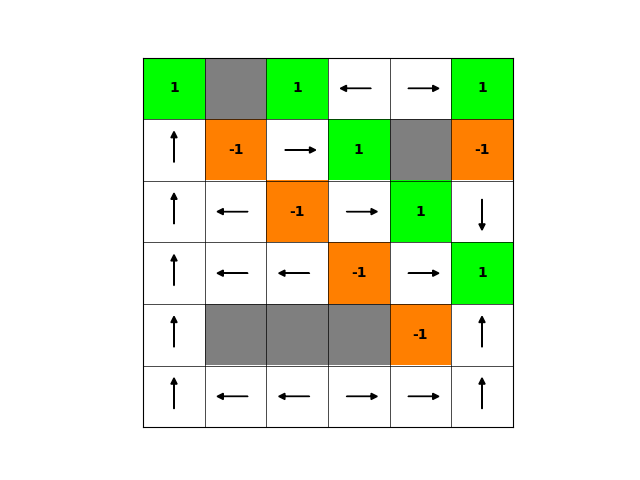
\includegraphics[width=100mm]{../asset/value_iteration_policy.png}
    \caption{Optimal policy for the gridworld environment. The arrows indicate the action to be taken in each state. The color of the arrows represent the value of the action.}
    \label{fig:value_iteration_policy}
\end{figure}

\subsection{Utility of all states}

\begin{figure}[H]
    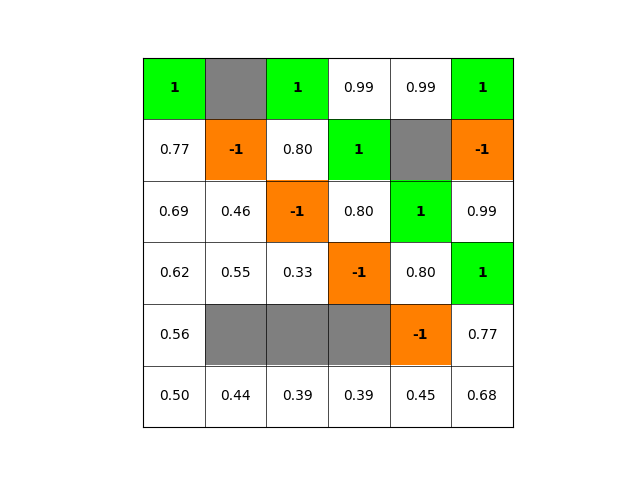
\includegraphics[width=100mm]{../asset/value_iteration_utility.png}
    \caption{Utility of all states in the gridworld environment. The color of the cells represent the value of the state.}
    \label{fig:value_iteration_utility}
\end{figure}

The more detailed value for the final utility is:

\begin{table}[H]
    \begin{tabular}{|l|l|l|l|l|l|}
        \hline
        0.0        & 0.0        & 0.0        & 0.99445061 & 0.98753071 & 0.0        \\\hline
        0.77247503 & 0.0        & 0.8        & 0.0        & 0.0        & 0.0        \\\hline
        0.68529708 & 0.4611854  & 0.0        & 0.8        & 0.0        & 0.99445061 \\\hline
        0.61840233 & 0.54986211 & 0.33239009 & 0.0        & 0.8        & 0.0        \\\hline
        0.56078941 & 0.0        & 0.0        & 0.0        & 0.0        & 0.77247503 \\\hline
        0.49686767 & 0.4406518  & 0.38504299 & 0.3947778  & 0.45040336 & 0.68411722 \\\hline
    \end{tabular}
\end{table}

\subsection{Convergence of value iteration}

\begin{figure}[H]
    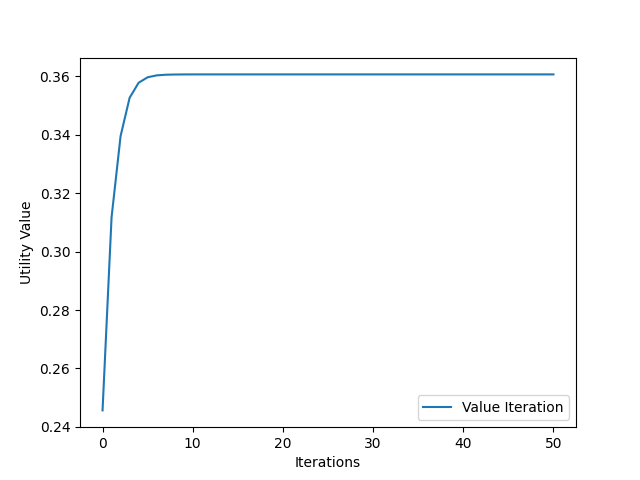
\includegraphics[width=100mm]{../asset/value_iteration_curve.png}
    \caption{Convergence of value iteration. The y-axis represents the maximum change in utility values across all states. The x-axis represents the number of iterations.}
    \label{fig:value_iteration_convergence}
\end{figure}

\section{Method of policy iteration}

\subsection{Description of Implemented Solution}

\paragraph{Initialization:} The setting is basically same with value iteration. Except here we initialize the policy as all actions are set to move right (0, 1).

\paragraph{Policy Evaluation:} For each state, the expected utility is computed based on the current policy's action, considering the probability of transitions to all possible next states and the corresponding rewards.

\paragraph{Policy iteration:} The iteration consists of two steps: evaluation and improvement.

Policy Evaluation: 
\[V^\pi (s) = \sum_{s', r} P(s', r|s, \pi(s))[r + \gamma V^\pi (s')] \]

where $V^\pi(s)$ is the utility of state $s$ under policy $\pi$, $P(s', r | s, \pi(s))$ is the probability of transitioning to state $s'$ with reward $r$ from state $s$ when following policy $\pi$. $\gamma$ is the discount factor and $\pi(s)$ is the action prescribed by policy $\pi$ in state $s$.

Policy Improvement:
\[\pi ' (s) = arg max_a \sum_{s', r} P(s', r|s, a)[r + \gamma V^\pi (s')] \]

where $pi '(s)$ is the updated action for state $s$ under the improved policy $\pi '$, $argmax_a$ denotes the action that maximizes the expected utility.

\paragraph{Termination:} The algorithm terminates when the policy is stable (The maximum change in utility values across all states $\delta$ is below a threshold, indicating that the utilities have converged).

\subsection{Plot of Optimal Policy}

\begin{figure}[H]
    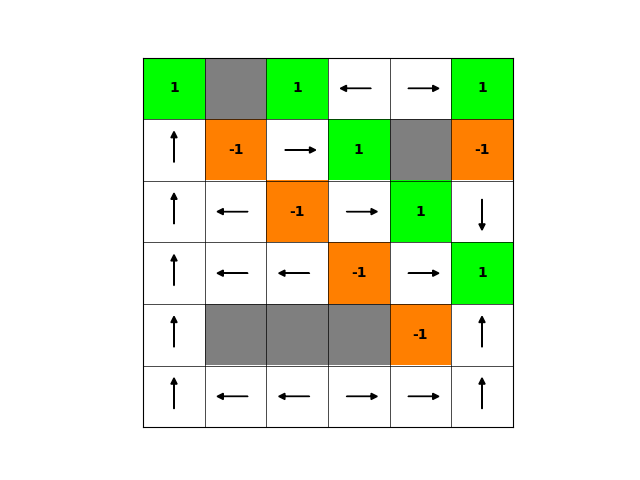
\includegraphics[width=100mm]{../asset/policy_iteration_policy.png}
    \caption{Optimal policy for the gridworld environment. The arrows indicate the action to be taken in each state. The color of the arrows represent the value of the action.}
    \label{fig:policy_iteration_policy}
\end{figure}

\subsection{Utility of all states}

\begin{figure}[H]
    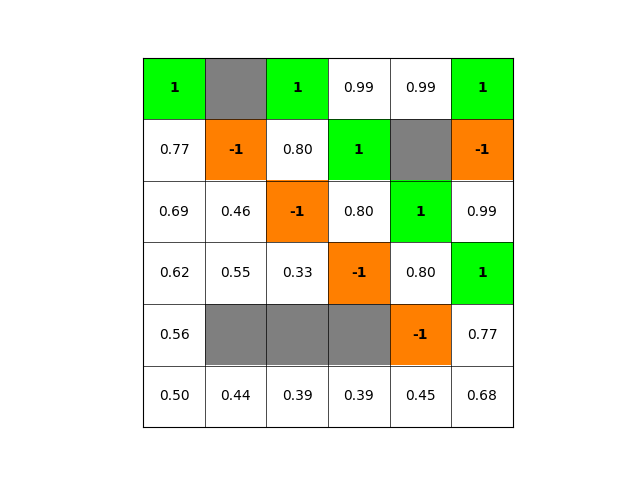
\includegraphics[width=100mm]{../asset/policy_iteration_utility.png}
    \caption{Utility of all states in the gridworld environment. The color of the cells represent the value of the state.}
    \label{fig:policy_iteration_utility}
\end{figure}

\subsection{Convergence of policy iteration}

\begin{figure}[H]
    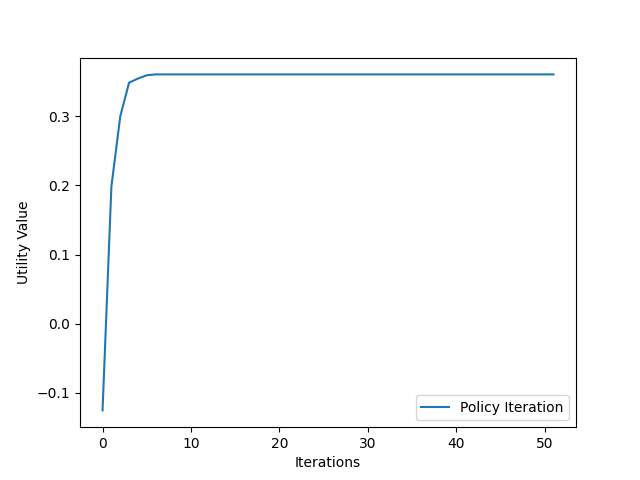
\includegraphics[width=100mm]{../asset/policy_iteration_curve.png}
    \caption{Convergence of policy iteration. The y-axis represents the maximum change in utility values across all states. The x-axis represents the number of iterations.}
    \label{fig:policy_iteration_convergence}
\end{figure}

\section{Bonus questions}

\end{document}
